\chapter{Modelli Stocastici: Script 6 e 7}

Per proiettare il valore del portafoglio nel futuro (un orizzonte di 120 mesi), i rendimenti medi passati sono insufficienti poiché non considerano il rischio di sequenza (la "sfortuna" di subire crolli all'inizio del PAC) né gli shock esogeni. \`E stato quindi implementato uno script R (\texttt{previsione\_7\_frontiera\_rischio.R}) basato sul \emph{Metodo Monte Carlo} e sulla scomposizione di Cholesky.

\section{Moto Browniano Geometrico (GBM)}
L'evoluzione del prezzo di un asset nel modello continuo \`e descritta dall'equazione differenziale stocastica (SDE):
\begin{equation}
dS_t = \mu S_t dt + \sigma S_t dW_t
\end{equation}
dove $dW_t$ è un processo di Wiener. Nel nostro modello discretizzato (su base mensile), il rendimento generato in un mese simulato per il portafoglio \`e guidato da shock estratti da una normale standard $\mathcal{N}(0,1)$.

\section{La Decomposizione di Cholesky}
Simulare N asset in modo indipendente sarebbe un errore fatale: le azioni tendono a crollare all'unisono e beni rifugio come l'oro tendono a muoversi in direzioni specifiche durante le crisi. Per forzare il modello stocastico a rispettare la struttura reale del mercato, la matrice di covarianza definita positiva $\Sigma$ viene fattorizzata in una matrice triangolare inferiore $L$:
\begin{equation}
\Sigma = L \cdot L^T
\end{equation}
Durante ogni step della simulazione Monte Carlo, un vettore di rumore bianco indipendente $Z \sim \mathcal{N}(0, I)$ viene moltiplicato per $L$, generando shock correlati $\epsilon$:
\begin{equation}
\epsilon = L \cdot Z
\end{equation}
Il rendimento generato in quel mese sar\`a quindi un vettore dipendente da $\mu$ mensile e dagli shock $\epsilon$ correlati.

\section{Dinamica Finanziaria nel Modello 7}
Nel Modello 7, la SDE stocastica \`e immersa in un ciclo \texttt{for} iterativo che, mese per mese, aggiorna il capitale $V_t$ applicando:
\begin{enumerate}
    \item \textbf{Inflazione (Deterioramento Nominale)}: Sottrazione di un coefficiente di svalutazione mensile (es. 2\% annuo diviso in 12), calcolando così il Capitale Reale.
    \item \textbf{Costi Sistemici (TER)}: Decurtazione di un fattore pari a $0.20\% / 12$ sul monte capitale gestito.
    \item \textbf{PAC (Dollar Cost Averaging)}: Iniezione vettoriale di nuova liquidit\`a, ponderata secondo i pesi del portafoglio (es. 60/20/20).
\end{enumerate}

\section{Limiti della Varianza e Misure Quantiliche (VaR e CVaR)}
La teoria classica Media-Varianza (su cui si fonda l'ottimizzazione di Markowitz) assume la varianza come misura universale del rischio. Tuttavia, questa assunzione presenta due limiti intrinseci: penalizza simmetricamente sia i rialzi che i crolli e fatica a catturare il rischio estremo delle "code grasse" (Fat Tails) della distribuzione. 

Per superare questo limite, l'approccio stocastico del Modello 7 sposta il focus sulle misure di rischio basate sui quantili della distribuzione delle perdite:
\begin{itemize}
    \item \textbf{Value at Risk (VaR)}: Calcola la perdita massima attesa in un orizzonte temporale dato, con un certo livello di confidenza (es. 95\%). È l'esatto quantile della probabilità di ricchezza futura.
    \item \textbf{Conditional Value at Risk (CVaR)}: Noto anche come \emph{Expected Shortfall}, risponde alla domanda fondamentale: "Se la perdita supera il limite del VaR, quanto sar\`a grave in media il disastro?". Calcola il valore atteso delle perdite relegate nel peggior 5\% degli scenari.
\end{itemize}

Per dimostrare empiricamente la necessità di abbandonare il calcolo parametrico puro del VaR (basato su $\mu + Z \cdot \sigma$), è stato eseguito un \emph{Test di Shapiro-Wilk} (Script 9) sui rendimenti storici del portafoglio reale. Sebbene in alcune combinazioni di ETF azionari diversificati l'ipotesi di normalità venga accettata, l'osservazione visiva (Figura \ref{fig:istogramma_normalita}) rivela costantemente che il VaR Storico (il quantile reale al 5\%) cade sempre più a sinistra rispetto al VaR Parametrico. La curva di Gauss sottostima sistematicamente il rischio estremo.

\begin{figure}[H]
    \centering
    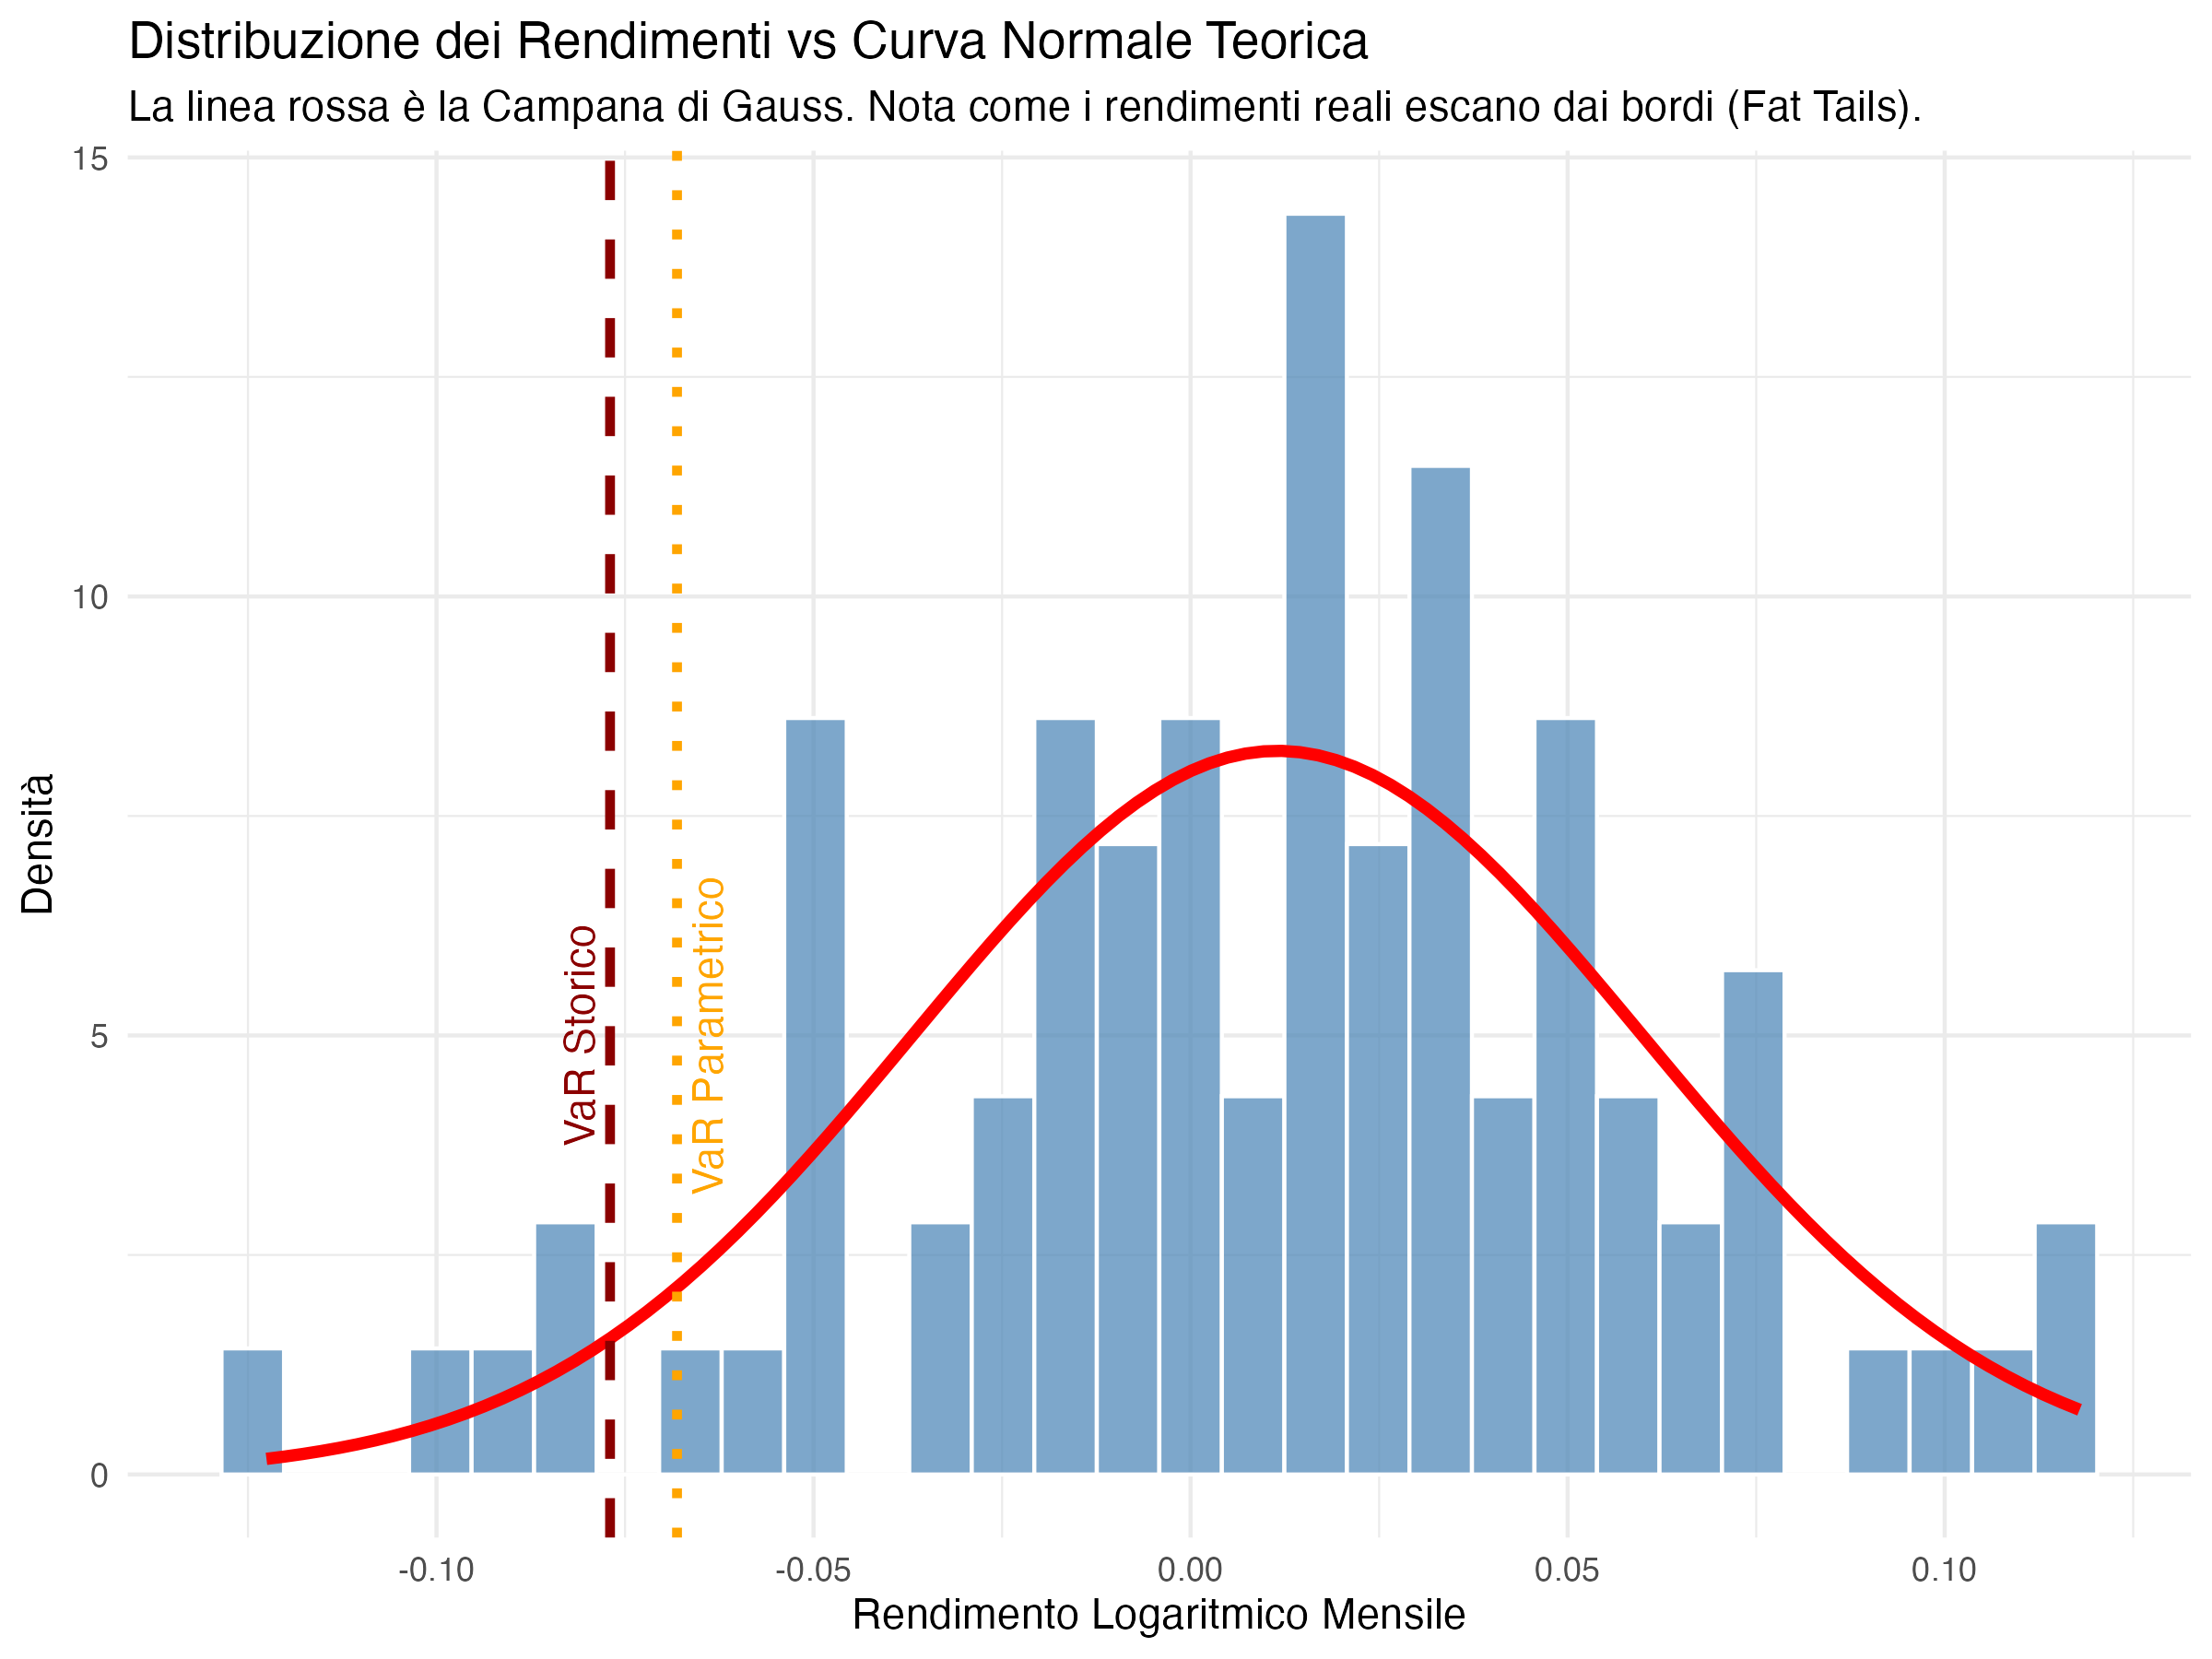
\includegraphics[width=0.9\textwidth]{immagini/istogramma_normalita.png}
    \caption{Test di Ipotesi e Confronto VaR: L'istogramma dei rendimenti reali a confronto con la Campana di Gauss teorica (rossa). Si nota come il VaR Storico (linea tratteggiata) si trovi a livelli di perdita superiori rispetto al VaR Parametrico, smascherando il limite della teoria Media-Varianza pura.}
    \label{fig:istogramma_normalita}
\end{figure}

\begin{figure}[H]
    \centering
    % \includegraphics[width=0.9\textwidth]{immagini/monte_carlo_plot.png}
    \vspace{6cm} % Spazio provvisorio in attesa dell'immagine
    \caption{Simulazione Monte Carlo: I percorsi stocastici generati dallo Script 7. La linea verde evidenzia la Mediana, la linea rossa il Worst-Case (CVaR).}
    \label{fig:monte_carlo}
\end{figure}

Il Modello 7 mostra in modo inequivocabile il ventaglio delle probabilità. Più la "nuvola" (funnel) di simulazione si allarga, maggiore è il rischio statistico del portafoglio. Il \emph{Conditional Value at Risk} (CVaR al 5\%) espresso numericamente nello script indica la media dei peggiori scenari, offrendo all'investitore l'esatto limite inferiore atteso in caso di cigno nero prolungato.
